\section{模拟分析}
根据式(\ref{equ:langzw}),单个布朗粒子在外势场下所满足的运动方程为:
$$
\dot{x}=-\frac{V^\prime\left( x_t,\lambda _t \right)}{\gamma}+\sqrt{2D}\xi _t
$$
其中,$\xi_t$为随机外力,如果仅在随机力作用下粒子随时间的变化将为高斯型分布,即为扩散的结果,也说明随机外力产生的是扩散运动;外势场的梯度对应着粒子的漂移运动,这个势场作为非禁闭势,将对粒子产生一定约束作用,形成一个存在的稳态分布$\gamma$代表摩擦对外力产生的减弱效应。

此处的运动方程形式上是常微分方程,但由于随机力存在,方程为一随机微分方程,需要考虑使用多粒子同时进行随机微分方程求解,其中随机力在对多粒子的平均中为0。同时考虑n个粒子,将粒子的坐标作为向量X,为使每个粒子方程都形式不变,将势场部分变成矩阵的对角元素,将随机力作为新的一个向量,即为:
$$
\dot{\vec{X}}=-\mathrm{diag}\frac{V^\prime\left( x_t,\lambda _t \right)}{\gamma}+\mathrm{diag}\sqrt{2D}\vec{\xi}_t
$$
其中$diag$表示将元素放在对角位置。
利用Euler–Maruyama方法\cite{vomscheidtKloedenPEPlaten1994},将随机微分方程在一定的时间区间上求解,我们可以得到每个粒子的运动过程,同时也能得到经过一定时间后,粒子在空间上的分布情况,如图(\ref{fig:sim-coordinate})所示。

\begin{figure}[htbp]
    \centering
    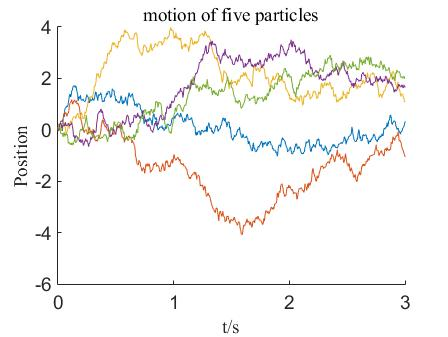
\includegraphics[width=0.8\linewidth]{figs/粒子坐标.jpg}
    \caption{前5个粒子的运动轨迹,模拟过程中选择$D=\gamma=\mathrm{k}_{0}T=1$,在$t_0=0.1 \text{s}$加入势场影响,时间间隔为0.005 s,粒子数$n=2000$。}
    \label{fig:sim-coordinate}
\end{figure}

在模拟中,我们选择势场$V$的形式为具有偏移的高斯型势场:
\begin{equation}
    V\left( x,\tau \right) =-A\left( \tau \right) e^{-\frac{\left( x-B\left( \tau \right) \right) ^2}{2}}
\end{equation}
为了验证之前所叙述的随机力对应扩散运动,同时还能在之后加入势场所产生的影响,我们选择$A(\tau)=\theta(\tau-t_0)$,其中$\theta$对应一个阶跃函数,表示在时间$t_0$之前没有势场影响,在$t_0$之后加入了势场的影响。为了能具体显示势场对漂移的影响,我们选择$B(\tau)=1$,可以直接展示势场对粒子运动的束缚作用。

\begin{figure}[htbp]
    \centering
    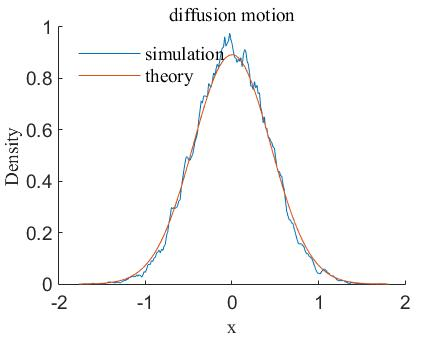
\includegraphics[width=0.8\linewidth]{figs/扩散运动.jpg}
    \caption{未加势场时,粒子的扩散运动。}
    \label{fig:sim-no-V}
\end{figure}

如图我们可以看到不加势场时,粒子运动为一扩散运动,形成高斯型分布,满足:
\begin{equation}
    \varrho \left( x,t \right) =\frac{1}{\left( 4\pi Dt \right) ^{1/2}}\exp \left[ -\frac{\left( x-x_0 \right) ^2}{4Dt} \right]
\end{equation}

需要注意其中势场有一个单位偏移,在此处才能看到分布的偏移情况。能在图 (\ref{fig:sim-V})中观察到中心位置处于1的位置上,势场对粒子的约束作用满足理论分布:

\begin{equation}
    \varrho \left( x,t \right) =Ce^{-\frac{x^2}{4Dt}-\frac{V\left( x,t \right)}{\mathrm{k}_{0}T}}
\end{equation}

其中$C$为不含$x$的归一化系数。

\begin{figure}[htbp]
    \centering
    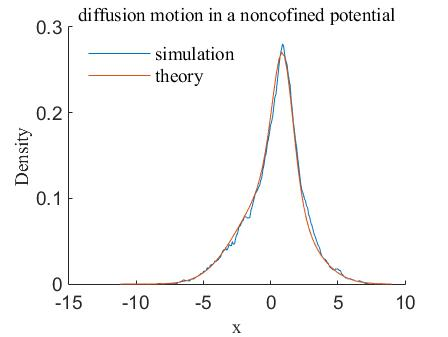
\includegraphics[width=0.8\linewidth]{figs/势场中的分布.jpg}
    \caption{加入势场后粒子的分布}
    \label{fig:sim-V}
\end{figure}